\hypertarget{parser_8hpp}{
\section{Dokumentacja pliku /home/pawel/Dokumenty/Uczelnia/grupappz/Source/Ass8-server/parser.hpp}
\label{parser_8hpp}\index{/home/pawel/Dokumenty/Uczelnia/grupappz/Source/Ass8-server/parser.hpp@{/home/pawel/Dokumenty/Uczelnia/grupappz/Source/Ass8-server/parser.hpp}}
}
{\tt \#include $<$boost/asio.hpp$>$}\par
{\tt \#include $<$string$>$}\par
{\tt \#include $<$fstream$>$}\par
{\tt \#include $<$libxml++/libxml++.h$>$}\par
{\tt \#include $<$libxml++/parsers/textreader.h$>$}\par
{\tt \#include \char`\"{}baza.hpp\char`\"{}}\par
{\tt \#include \char`\"{}debug.hpp\char`\"{}}\par


Wykres zależności załączania dla parser.hpp:\nopagebreak
\begin{figure}[H]
\begin{center}
\leavevmode
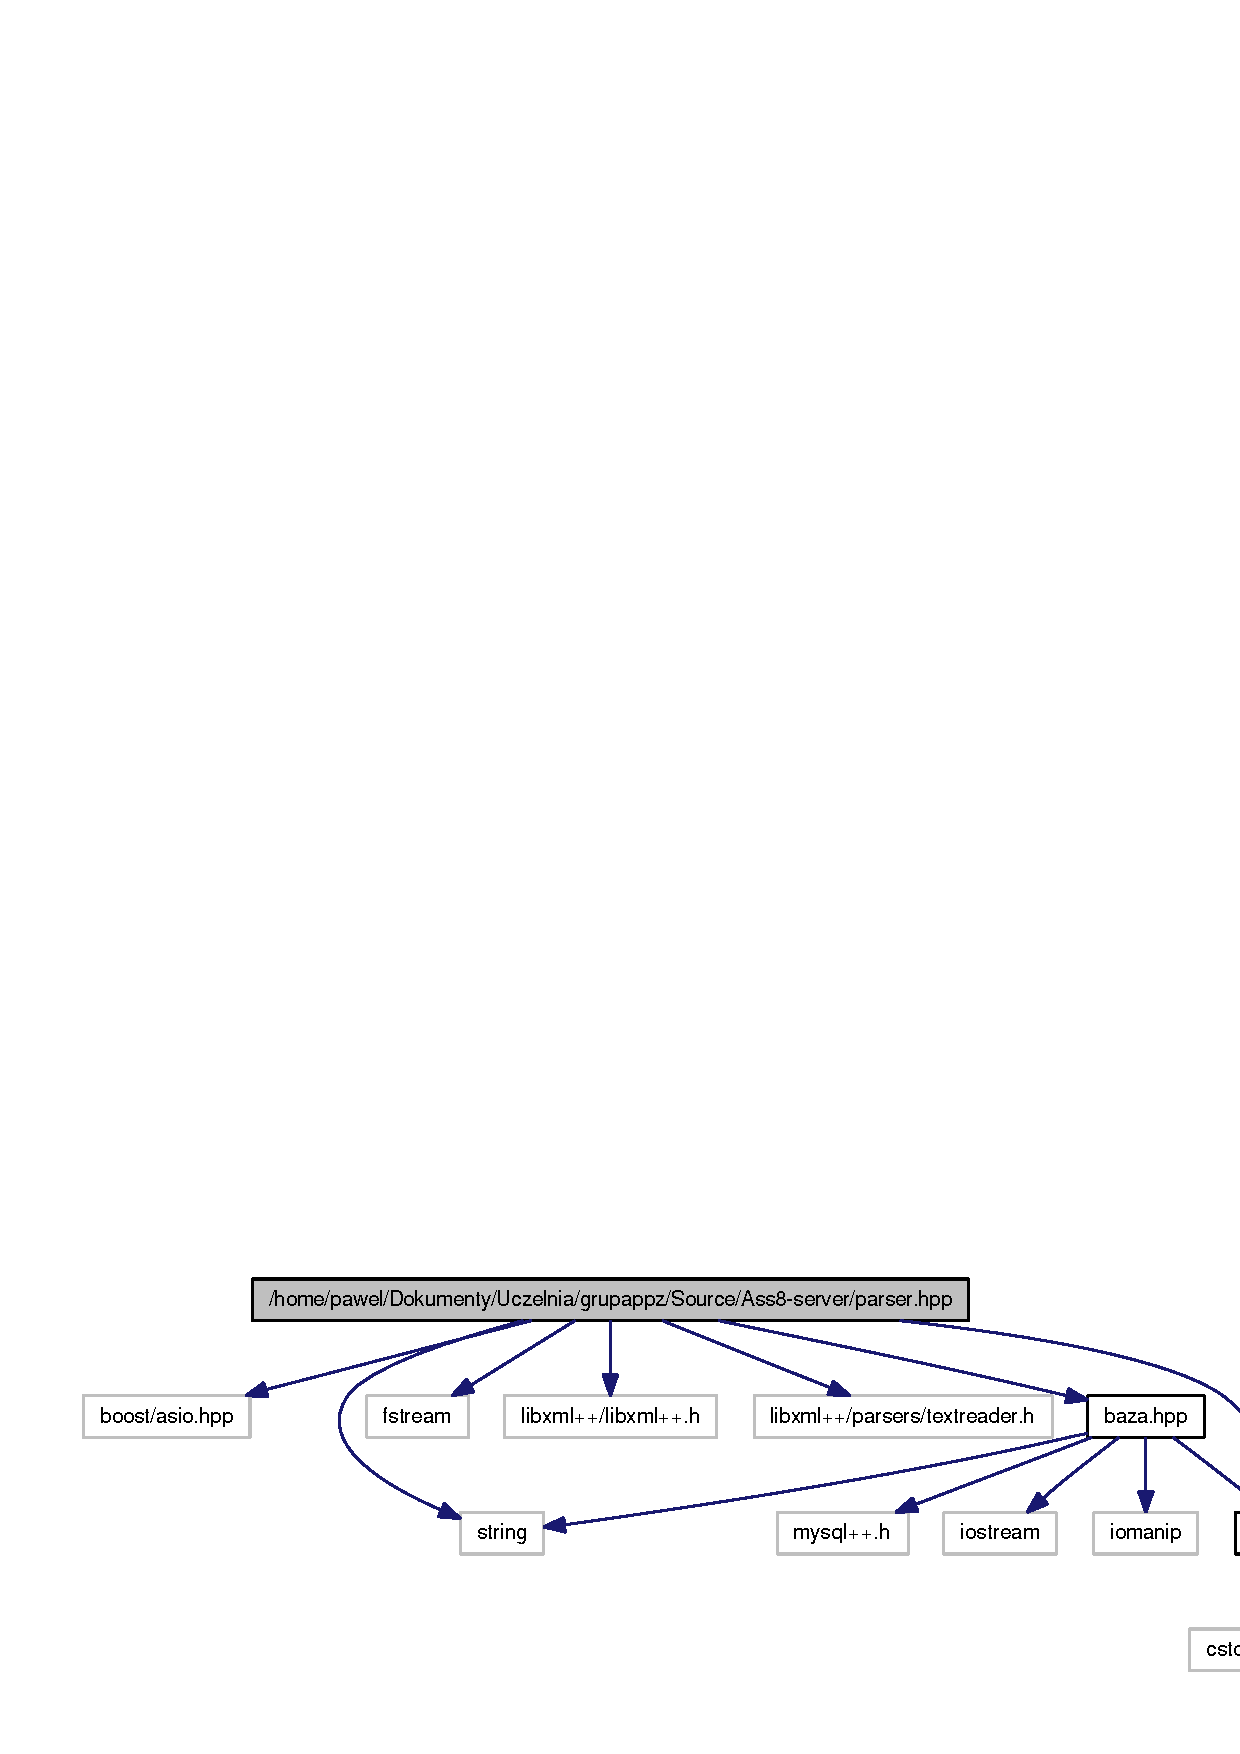
\includegraphics[width=339pt]{parser_8hpp__incl}
\end{center}
\end{figure}


Ten wykres pokazuje, które pliki bezpośrednio lub pośrednio załączają ten plik:\nopagebreak
\begin{figure}[H]
\begin{center}
\leavevmode
\includegraphics[width=372pt]{parser_8hpp__dep__incl}
\end{center}
\end{figure}
\subsection*{Komponenty}
\begin{CompactItemize}
\item 
class \hyperlink{classparser}{parser}
\end{CompactItemize}
\subsection*{Definicje}
\begin{CompactItemize}
\item 
\#define \hyperlink{parser_8hpp_eca034f67218340ecb2261a22c2f3dcd}{BUFSIZE}~1024
\item 
\#define \hyperlink{parser_8hpp_b46db07bcc5d1bb3dbc73f7be2592ee0}{BUFSIZE2}~1024$\ast$2
\end{CompactItemize}
\subsection*{Funkcje}
\begin{CompactItemize}
\item 
void \hyperlink{parser_8hpp_6c724feff242ad0cd599cdd458f73199}{eat\_\-zombie} ()
\end{CompactItemize}


\subsection{Dokumentacja definicji}
\hypertarget{parser_8hpp_eca034f67218340ecb2261a22c2f3dcd}{
\index{parser.hpp@{parser.hpp}!BUFSIZE@{BUFSIZE}}
\index{BUFSIZE@{BUFSIZE}!parser.hpp@{parser.hpp}}
\subsubsection[{BUFSIZE}]{\setlength{\rightskip}{0pt plus 5cm}\#define BUFSIZE~1024}}
\label{parser_8hpp_eca034f67218340ecb2261a22c2f3dcd}




Definicja w linii 19 pliku parser.hpp.\hypertarget{parser_8hpp_b46db07bcc5d1bb3dbc73f7be2592ee0}{
\index{parser.hpp@{parser.hpp}!BUFSIZE2@{BUFSIZE2}}
\index{BUFSIZE2@{BUFSIZE2}!parser.hpp@{parser.hpp}}
\subsubsection[{BUFSIZE2}]{\setlength{\rightskip}{0pt plus 5cm}\#define BUFSIZE2~1024$\ast$2}}
\label{parser_8hpp_b46db07bcc5d1bb3dbc73f7be2592ee0}




Definicja w linii 20 pliku parser.hpp.

\subsection{Dokumentacja funkcji}
\hypertarget{parser_8hpp_6c724feff242ad0cd599cdd458f73199}{
\index{parser.hpp@{parser.hpp}!eat\_\-zombie@{eat\_\-zombie}}
\index{eat\_\-zombie@{eat\_\-zombie}!parser.hpp@{parser.hpp}}
\subsubsection[{eat\_\-zombie}]{\setlength{\rightskip}{0pt plus 5cm}void eat\_\-zombie ()}}
\label{parser_8hpp_6c724feff242ad0cd599cdd458f73199}




Here is the caller graph for this function:\nopagebreak
\begin{figure}[H]
\begin{center}
\leavevmode
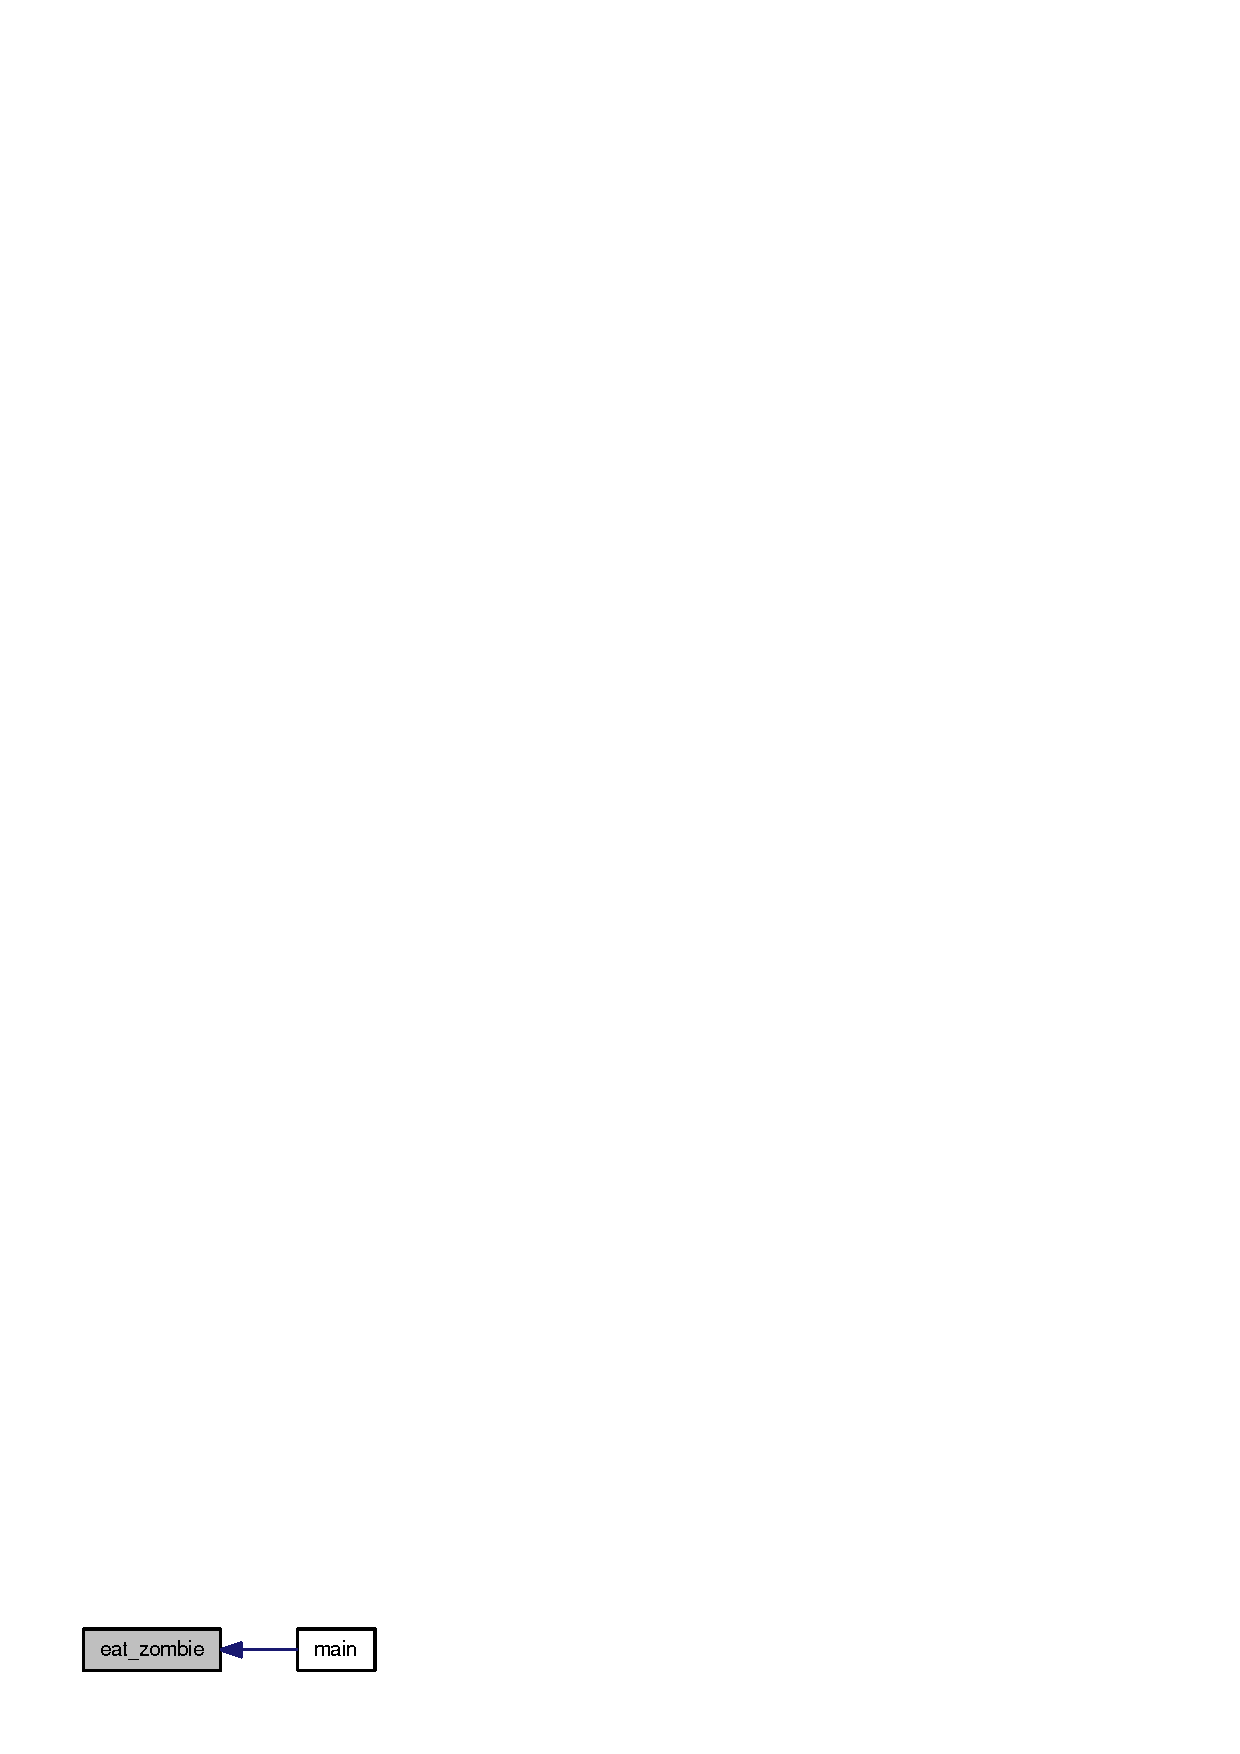
\includegraphics[width=92pt]{parser_8hpp_6c724feff242ad0cd599cdd458f73199_icgraph}
\end{center}
\end{figure}
